\documentclass[10pt,a4paper]{article}

% ─── Packages ─────────────────────────────────────────

\usepackage{fontspec}
\setmainfont{Times New Roman}

\usepackage[top=0.6cm,bottom=0.5cm,left=1.45cm,right=1.45cm]{geometry}

\usepackage{titlesec}
\usepackage{enumitem}
\usepackage{hyperref}
\usepackage{xcolor}
\usepackage{tabularx}
\usepackage{graphicx}
\usepackage{parskip}

% ─── Colors ───────────────────────────────────────────

\definecolor{primary}{RGB}{30,40,90}
\definecolor{namecolor}{RGB}{0,120,180}
\definecolor{accent}{RGB}{50,90,150}
\definecolor{rulecol}{RGB}{200,205,220}
\definecolor{gray}{RGB}{90,90,90}

\hypersetup{
    colorlinks=true,
    urlcolor=accent
}

\pagestyle{empty}
\setlength{\parskip}{0pt}

% ─── Section ──────────────────────────────────────────

\titleformat{\section}
    {\normalsize\bfseries\color{primary}}
    {}
    {0em}
    {}
    [\vspace{1pt}\textcolor{rulecol}{\titlerule[0.6pt]}\vspace{1pt}]

\titlespacing{\section}{0pt}{3pt}{1pt}

% ─── Entry ────────────────────────────────────────────

\newcommand{\entry}[3]{%
    \noindent
    \begin{tabularx}{\linewidth}{X r}
        \textbf{\color{primary}#1} &
        {\scriptsize\color{gray}#2}
    \end{tabularx}\\[-2pt]
    {\scriptsize\textit{\color{gray}#3}}
    \vspace{0.5pt}
}

% ─── Compact list ─────────────────────────────────────

\newenvironment{cvitems}{
    \begin{itemize}[
        leftmargin=1.1em,
        topsep=0pt,
        itemsep=0.3pt,
        parsep=0pt,
        partopsep=0pt
    ]
}{
    \end{itemize}
}

% ═════════════════════════════════════════════════════

\begin{document}

% ─── HEADER ───────────────────────────────────────────

\noindent

\begin{tabularx}{\linewidth}{@{}X r@{}}

\begin{minipage}[c]{\linewidth}

    {\LARGE\bfseries\color{namecolor} Ho Huynh Nhu}\\[1pt]

    {\large\bfseries\color{primary}
    Industrial Engineering (IE) Staff}\\[2pt]

    {\scriptsize\color{gray}
    20/10/2003
    \enspace\textcolor{rulecol}{|}
    \enspace (+84) 367 503 477
    \enspace\textcolor{rulecol}{|}
    \enspace
    \href{mailto:hhnhu2003@gmail.com}{hhnhu2003@gmail.com}
    \enspace\textcolor{rulecol}{|}
    \enspace Ho Chi Minh City}\\[1pt]

    {\scriptsize
    \href{https://github.com/hohuynhnhu}
    {github.com/hohuynhnhu}
    \enspace\textcolor{rulecol}{|}
    \enspace
    \href{https://www.facebook.com/huynhnhu.ho.961}
    {facebook.com/huynhnhu.ho.961}
    }

\end{minipage}

&

\begin{minipage}[c]{2.1cm}
    \raggedleft
    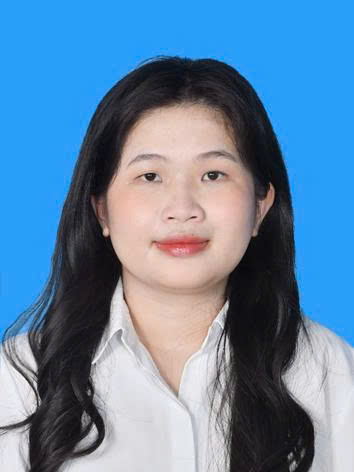
\includegraphics[
        width=2.1cm,
        height=2.5cm,
        keepaspectratio
    ]{assets/avt.jpg}
\end{minipage}

\end{tabularx}

\vspace{1pt}

\textcolor{rulecol}{\rule{\linewidth}{0.6pt}}

% ─── CAREER OBJECTIVE ─────────────────────────────────

\section*{Career Objective}

{\small
Final-year Information Technology student seeking an IE Staff position in the
garment industry. Experienced in collecting and analyzing data, tracking
operational metrics, recording incidents and their causes, preparing quick
reports with Excel and Power BI, and analyzing video with AI. A fast learner
who adapts well to new environments, eager to learn and apply IE methods such
as operation time study, line balancing, and productivity improvement.
}

% ─── EDUCATION ────────────────────────────────────────

\section*{Education}

\entry
{University of Transport Ho Chi Minh City (UTH)}
{10/2022 -- 10/2026}
{Bachelor of Information Technology -- Completed coursework}

{\small
\begin{cvitems}

    \item GPA: \textbf{3.4 / 4.0}

    \item \textbf{Excellent Scholarship} -- Semester 1, 2025

    \item \textbf{Second Prize -- AI Track},
    UTH Student Scientific Research Conference 2025

\end{cvitems}
}

% ─── SKILLS ───────────────────────────────────────────

\section*{Skills}

{\small

\begin{tabularx}{\linewidth}{@{}lX@{}}

\textbf{Office Computing}
&
Excel (Pivot Table, Lookup Functions, Charts, Data Filtering \& Summarizing),
Power BI, Regular Reporting
\\[1pt]

\textbf{Data Collection \& Analysis}
&
Data Collection, Data Cleaning \& Validation, Trend Analysis,
KPI Analysis, Root-cause Investigation, Data Visualization
\\[1pt]

\textbf{Monitoring \& Incident Handling}
&
Real-time Metric Tracking, Anomaly Detection,
Error Logging \& Resolution, Quick Reporting
\\[1pt]

\textbf{Video / Image Analysis}
&
YOLO, MediaPipe, CNN, Video Processing, Image Preprocessing
\\[1pt]

\textbf{Programming \& Data}
&
Python, Pandas, NumPy, SQL, PostgreSQL, ETL, Apache Airflow
\\[1pt]

\textbf{Tools}
&
Jira, Confluence, Git, Docker, Postman, VS Code

\end{tabularx}

}

% ─── WORK EXPERIENCE ──────────────────────────────────

\section*{Work Experience}

\entry
{Gotik Consulting -- Data Engineer}
{Python \textbar{} dbt \textbar{} PostgreSQL \textbar{} Airflow \textbar{} Power BI}
{03/2026 -- 05/2026}

{\small
\begin{cvitems}
    \item Monitored hourly ETL workflows on Apache Airflow: logged failures, investigated causes, and resolved them to keep the system running continuously and minimize interruption time.

    \item Built Power BI dashboards to track operational metrics and prepared regular reports to help management make data-driven decisions.

    \item Wrote SQL queries to aggregate, filter, and join data, ensuring reliable figures for reports.

    \item Processed, checked, and standardized Odoo business data to detect discrepancies and prepare accurate datasets for analysis.
\end{cvitems}
}

% ─── PROJECTS ─────────────────────────────────────────

\section*{Featured Projects}

\entry
{VehicleScan -- Vehicle Recognition \& Monitoring System}
{Python \textbar{} YOLO \textbar{} CNN \textbar{} Siamese Network \textbar{} ESP32 \textbar{} Kafka}
{03/2025 -- 03/2026}

{\small
\begin{cvitems}
    \item Built an AI-based vehicle recognition system combined with IoT sensors (ESP32) to monitor parking in real time.
    \item Processed image and sensor data and integrated it into one centralized system to track operating status and support reporting.
    \item GitHub: \href{https://github.com/LeKhang-cn22h/VehicleScanner}{VehicleScanner}
\end{cvitems}
}

\vspace{1pt}

\entry
{Fall Detection -- Video Analysis System for Fall Detection}
{Python \textbar{} PyTorch \textbar{} YOLOv8 Pose \textbar{} MediaPipe \textbar{} Transformer}
{04/2026 -- 06/2026}

{\small
\begin{cvitems}
    \item Analyzed video to extract human pose using MediaPipe and YOLOv8 Pose and detect fall incidents.
    \item Achieved 97.8\% mean accuracy with 5-fold cross-validation and tested on unseen data.
\end{cvitems}
}

\vspace{1pt}

\entry
{Delivery Driver -- Order Analytics System}
{Python \textbar{} SQL \textbar{} Kafka \textbar{} PostgreSQL \textbar{} MinIO}
{12/2025 -- 02/2026}

{\small
\begin{cvitems}
    \item Built an automated data pipeline to collect and process order data for analysis.
    \item Applied RFM and Association Rule Mining to analyze customer behavior, generating insights to support service-point optimization.
    \item GitHub: \href{https://github.com/LeKhang-cn22h/BE-delivery-driver}{BE-delivery-driver}
\end{cvitems}
}

% ─── ADDITIONAL INFORMATION ───────────────────────────

\section*{Additional Information}

{\small

\begin{tabularx}{\linewidth}{@{}lX@{}}

\textbf{Soft Skills}
&
Fast learner, adaptable \textbar{} Meticulous, responsible \textbar{}
Teamwork \textbar{} Quick, clear reporting

\\[1pt]

\textbf{English}
&
Technical document reading and basic communication

\\[1pt]

\textbf{Availability}
&
Available for full-time IE Staff opportunities.

\end{tabularx}

}
\end{document}